In this section there will be described expected project behavior and resulting requirements. 
Requirements can be divided into two categories - functional and non-functional. 
Functional ones describe what should product do, its specific behavior or function.
On the other hand non-functional requirements cover what product is.

\section{Description}
To clarify and properly explain life cycle of one run of server side application, its usage and possible requirements, structure of UML's sequential diagram was adopted. 
As there was a need to express even a physical gestures (like raising hand with mobile there), diagram might violate some of sequential diagram rules.
Therefore we show in figure \ref{img:wholeapp_seq} interaction between all actors and their mobile devices.

\begin{figure}[!h]
    \begin{center}
    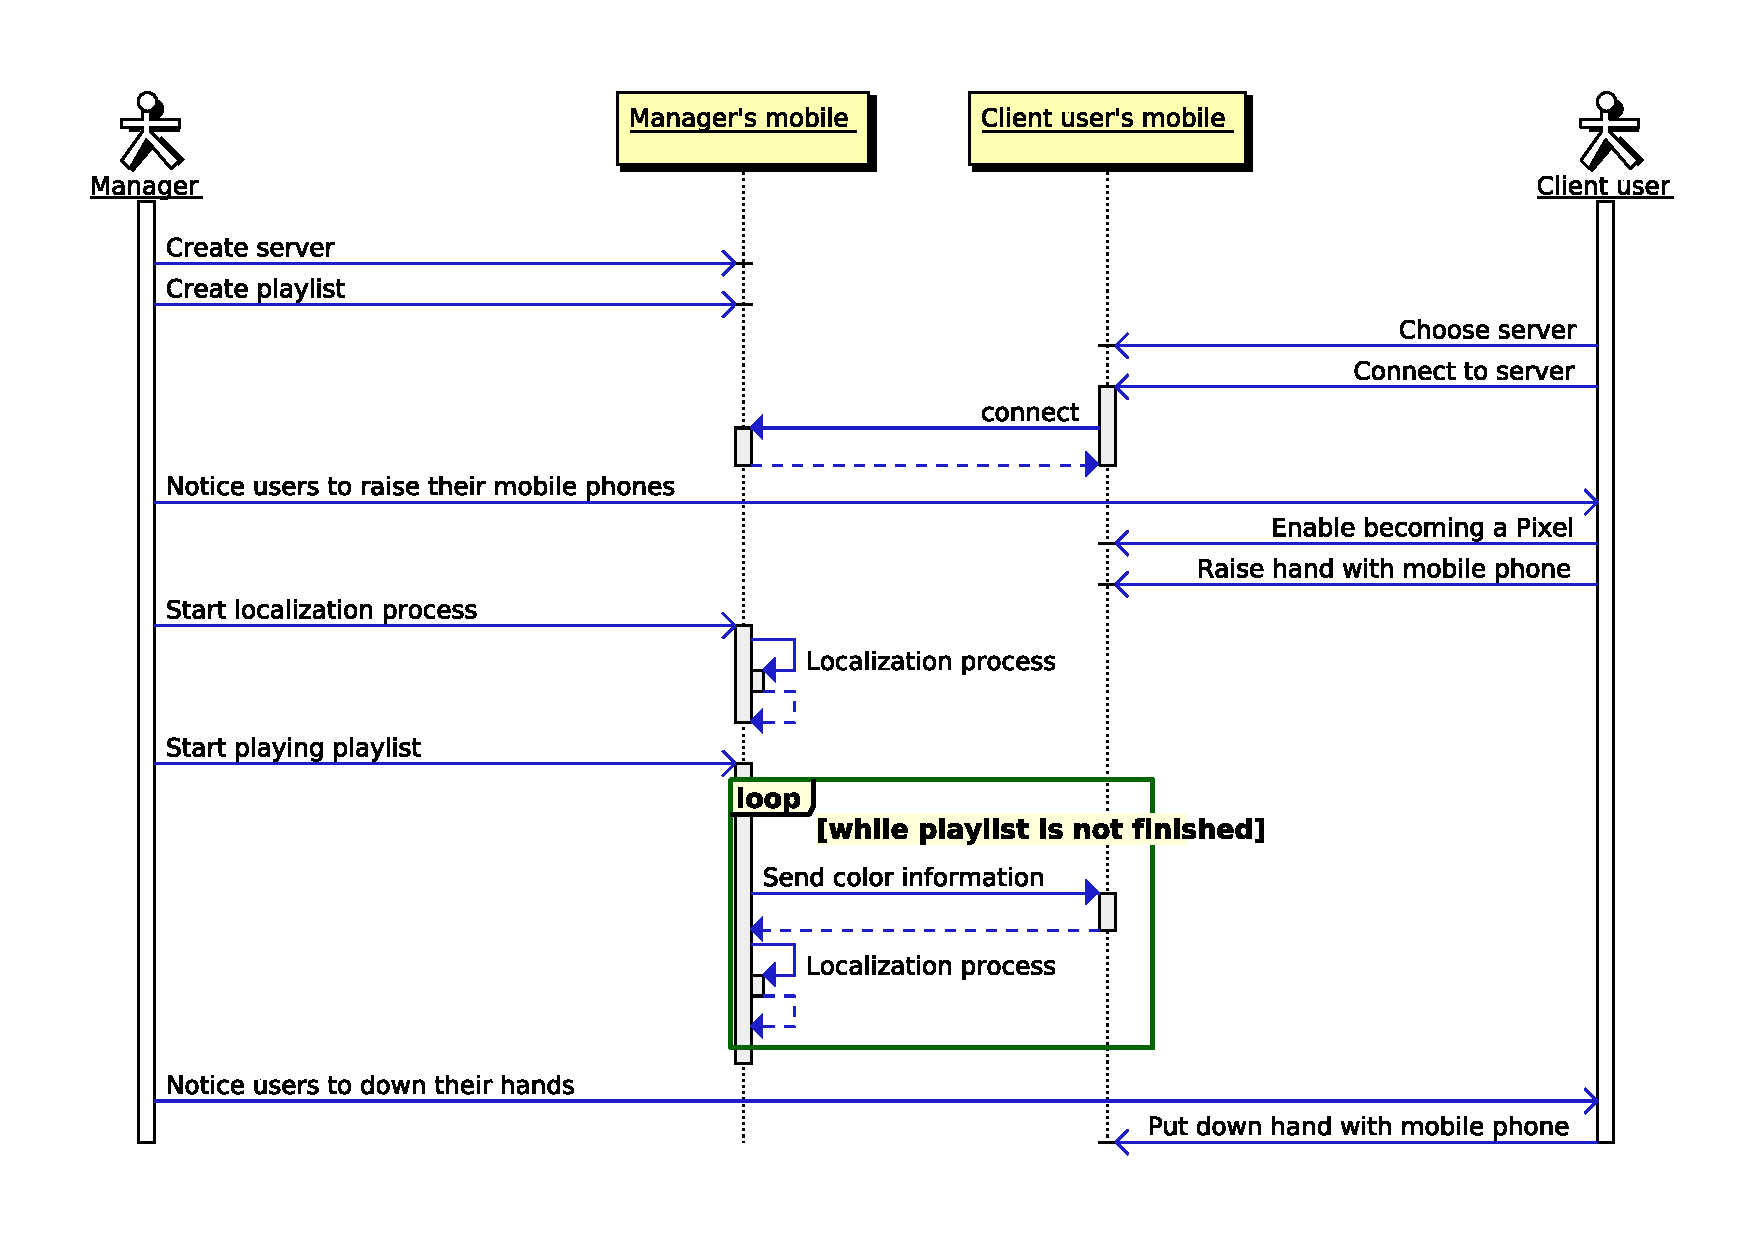
\includegraphics[scale=0.4]{images/wholeapp_seq.pdf}
    \caption{Sequential diagram depicting basic scenario of using product with all actors.}
    \label{img:wholeapp_seq}
    \end{center}
\end{figure}


\section{Use case diagram}
As we have defined terminology in section \ref{sec:terminology} we will use actor's names according to that terminology.
In the figure bellow is shown use case diagram \ref{img:usecase} of the whole system.

\begin{figure}[!h]
    \begin{center}
    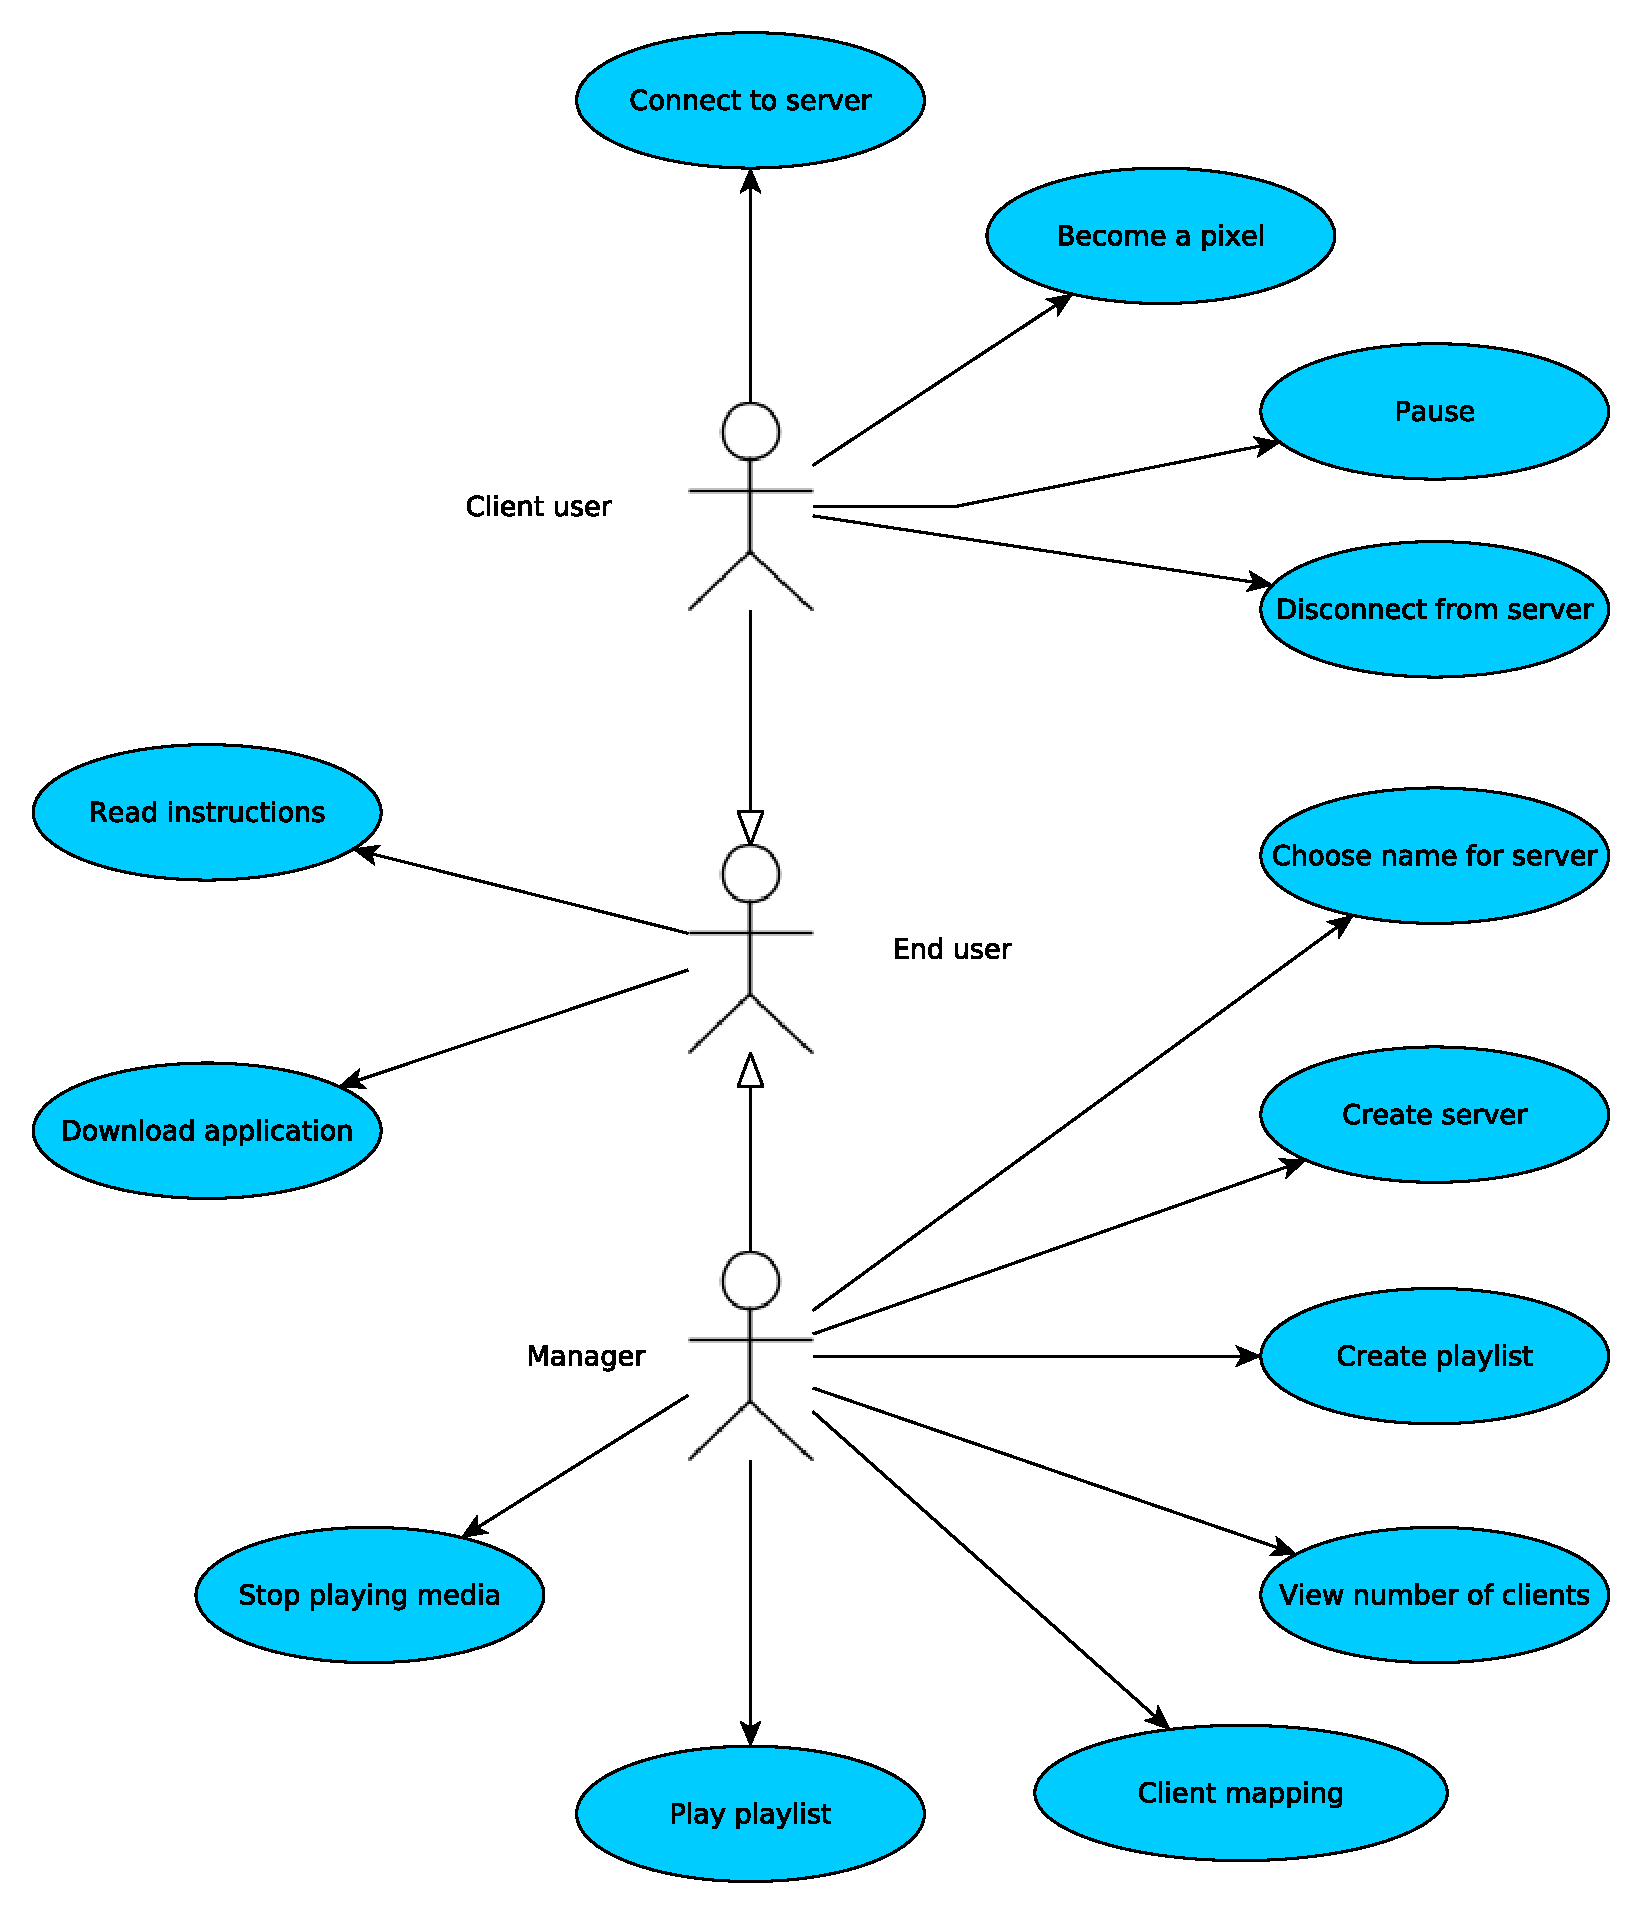
\includegraphics[scale=0.4]{images/usecase.pdf}
    \caption{Use case diagram depicting all actors.}
    \label{img:usecase}
    \end{center}
\end{figure}

\section{Requirements}
According to use case diagram \ref{img:usecase}, requirements were created.


\subsection{Functional}
You can see list of functional requirements from end user's point of view below.
\begin{enumerate}
	\item[\textbf{E1}] \label{req_E1}
		I as a end user want to be able to read instructions.
		
	\item[\textbf{E2}] \label{req_E2}
		I as a end user want to be able to download relevant application from mobile application store.
\end{enumerate}

You can see list of functional requirements from client user's point of view below.
\begin{enumerate}
	\item[\textbf{C1}] \label{req_C1}
		I as a client user I want to easily choose to which server/concert stage I would like to connect.
		
	\item[\textbf{C2}] \label{req_C2}
		I as a client user I want to connect to chosen server.
		
	\item[\textbf{C3}] \label{req_C3}
		I as a client user I want to become a \emph{Pixel}.
	
	\item[\textbf{C4}] \label{req_C4}
		I as a client user I want to be able to pause being a Pixel.
		
	\item[\textbf{C5}] \label{req_C5}
		I as a client user I want to be able to disconnect from server/stage.
\end{enumerate}


You can see list of functional requirements from manager's point of view below.
\begin{enumerate}
	\item[\textbf{M1}] \label{req_M1}
		I as a manager I want to be able to choose name for my server/stage.
		
	\item[\textbf{M2}] \label{req_M2}
		I as a manager I want to be able to create a server.
		
	\item[\textbf{M3}] \label{req_M3}
		I as a manager I want to be able view attendance.
	
	\item[\textbf{M4}] \label{req_M4}
		I as a manager I want to be able to start mobile phone localization.
		
	\item[\textbf{M5}] \label{req_M5}
		I as a manager I want to be able to choose playlist to be played.
		
	\item[\textbf{M6}] \label{req_M6}
		I as a manager I want to be able to start playing given media.
		
	\item[\textbf{M7}] \label{req_M7}
		I as a manager I want to be able to start pause playing the media.
	\item[\textbf{M8}] \label{req_M8}
		I as a manager I want to be able to start pause stop the media.
\end{enumerate}

\subsubsection{Detailed use cases}
In this section there will be described some use cases in detail.
\begin{table*}[!h]
	\def\arraystretch{1.25}
	\caption{Use case detail: Create playlist}
	\label{tab:usecase1}
	
	\begin{tabular}{p{\textwidth}}
		\toprule
		\textbf{Use case detail: Create playlist} \\
		\midrule
		Actors: Manager \\
		Conditions:
		\begin{enumerate}
			\item Manager had created server.
		\end{enumerate}
		Events flow:
		\begin{enumerate}
			\item Use case starts when manager choose option "Create playlist".
			\item Application will display list of possible media (videos, images) that can be played.
			\item Manager can preview specific media (view on his own screen).
			\item Manager chooses media to be played, order of choosing will be order of playing.
			\item Manager confirms the playlist.
			\item Use case ends.
		\end{enumerate}
		Alternative flow:
		\begin{enumerate}
			\item Manager can quit the screen and return to main menu anytime.
		\end{enumerate}
%		\\ 
		\vspace{0.6em}
		\hrule
%		\\[0.1pt]
%		\bottomrule[1mm]
	\end{tabular}
\end{table*}

\subsection{Non-functional}
You can see non-functional requirements listed below.

\begin{enumerate}
\item[\textbf{N1}] \label{req_N1} Product must work as a server and client architecture.
\item[\textbf{N2}] \label{req_N2} Client side application must work on at least one mobile platform.
\item[\textbf{N3}] \label{req_N3} Application must be deployed to relevant mobile application store.
\item[\textbf{N4}] \label{req_N4} The product must be scalable - it must work with different count of mobile phones.
\item[\textbf{N5}] \label{req_N5} The product must be prepared for future using outside of rock concert domain.
\item[\textbf{N6}] \label{req_N6} Final product must be finished until 21st of November 2013 and presented to the committee and the customer.
\end{enumerate}

\section{Summary}
In this chapter was explained how the application's basic life-cycle may look like and was introduced Use case diagram.
According to Use case diagram there were created \emph{Epics} which serve as a requirements. 
After that non-functional requirements were introduced.
In following chapters each user story which is connected to relevant requirement will be referenced with requirement's identification.

As you could see, end user's interaction with both applications is rather simple (and as our customer suggested the user interface is not core of the work) the main attention will be focused on image processing and network programming.